% Sample file on how to use subfiles.
\documentclass[MikaelDissertation.tex]{subfiles}

\begin{document}

\chapter{Introduction}

\section{The process of sintering of hardmetal}

Manufacturing of PM products is based on the ``welding'' (sintering) of particles due to heating or combined heating and mechanical loading (uniaxial or isotropic pressing).
To model and simulate the sintering of hard metals, typically WC with Co as the binder metal in the case of a WC-Co-Ti-C system, is particularly challenging in view of the fact that the sintering process involves both solid and melt states of the constituents.
In brief, the manufacturing process can be split into three different sequential stages:
(I) Compaction of powder compound, with initially around \SI{70}{\percent} porosity, into a ``green body'' with roughly \SIrange{20}{40}{\percent} porosity.
(II) Heating in oven up well above the melting temperature for Co (ca \SI{1500}{\celsius}).
(III) Cooling to room temperature.

The purpose is to achieve net-shape already of the green body, whereby the subsequent sintering would result mainly in change of volume (without distortion, i.e. shear deformation).
Since uniaxial pressing is normally used for the initial compaction of hard metal, it is likely that wall friction leads to inhomogeneous
distribution of residual stresses and bulk density in the green body (at least to some extent).
This is an unwanted effect that obscures the goal of net-shape.

During the heating phase, thermal expansion is combined with a certain amount of solid state sintering before melting of the binder, which is necessary in order to achieve ``liquid-phase'' sintering.
During the hold-time at the given temperature, significant compaction (densification, consolidation) takes place due to a combination of solid deformation, diffusion and liquid motion, which brings about reduced porosity.
The so-called ``sintering stress'', which is a macro-scale manifestation of the surface tension between the constituents and the pores, is the ``driving force'' for compaction; hence, sintering can take place under zero external load of the specimen (known as ``free sintering'').
However, the residual stresses after compaction will effect the process.

\textbf{Remark:} It is possible to achieve a sintered product below or above the melting temperature of the Co-binder.
Up to \SI{80}{\percent} of the densification can be achieved in pure solid state sintering, although a completely dense product can only be achieved with liquid phase.
These two cases are often denoted solid and liquid state sintering, respectively, in the literature.

% There are generally two characteristic stages in terms of porosity characteristics:
% At the early stage of sintering all pores are connected, which leads to quite rapid densification, in particular due to viscous flow of the liquid binder. Later on, within a certain temperature interval, all binder has solidified and the (possibly remaining) pores are closed off (and isolated) into near-equilibrium, which leads to much lower rate of consolidation.

Clearly, the aim of the process is that the final product is completely dense, i.e. there is no rest-porosity, with no net-shape distortion.
This may be hard to accomplish if the green body bulk density is severely inhomogeneous and/or the liquid phase sintering is inefficient (in terms of insufficient amount of binder phase and/or incomplete melting).

\section{Modeling and simulation efforts --- A brief review}

A wealth of literature deals with the modeling and simulation of the sintering process.
Primarily, this relates to the constitutive modeling of
(1) the powder material response for green body (pre)compaction and 
(2) the high temperature response and sintering mechanisms pertinent to both solid and liquid phase sintering.
Modeling efforts can be classified by two major paradigms: \emph{a priori macroscale modeling} and \emph{micromechanics modeling and computational homogenization}.

\subsection{Macroscale modeling}
\textbf{update!}

A vast majority of the existing literature on \emph{a priori} macro-scale modeling is devoted to the compaction stage, and it is noted that very few (if any) attempts have been made to develop a unifying macroscopic constitutive model for the compaction and sintering stages.
As to the compaction process, material rate-independence (elasto-plasticity) is a common (and valid) assumption.
Such plasticity models are often taken, at least conceptually, from soil mechanics.
The major focus is on the evolution of the yield surface due to changing porosity as the predominant hardening mechanism, e.g.\ Fleck et al.\ \cite{fleck_yielding_1992},
Oliver et al.\ \cite{oliver_plasticity_1996}, Brandt and Nilsson \cite{brandt_fe-simulation_1998}, Redanz \cite{redanz_numerical_1998}, Kraft \cite{kraft_optimizing_2003}.

For the solid phase sintering, the major feature is the strong rate-dependence close to, and above, the melting temperature of the binder.
Models based on viscoelasticity and viscoplasticity have, therefore, been proposed to simulate the creep behavior of the highly deformable (and even partly melt) binder, e.g. Shinagawa \cite{shinagawa_finite_1996}, Brandt and Nilsson \cite{brandt_fe-simulation_1998}.
Clearly, it is of utmost importance to model the high sensitivity of yield stress to temperature, e.g. Mähler et al.\ \cite{mahler_modelling_2000}.
The task of providing a rational thermodynamic definition of the sintering stress was addressed by, e.g. Reid and Oakberg \cite{reid_continuum_1990}, Mähler and Runesson \cite{mahler_constitutive_2003}.

As to liquid phase sintering, the text-book by German \cite{german_sintering_1996} is still an authority in the field.
Examples of the rich literature are Svoboda et al.\ \cite{svoboda_model_1996}, Xu and Mehrabahdi \cite{xu_micromechanical_1997}, Lu et al.\ \cite{lu_porosity_2001}, who used a single-phase approach.

% To date, it seems that no attempts have been made in the literature to use mixture theory, which explicitly acknowledges the coexistence of a solid skeleton of the WC-particles and partly solidified and liquid Co.

\subsection{Micromechanics modeling and computational homogenization}

Most micromechanically based models consider idealized geometrical arrangement, such as a regular array of spheres, within a Representative Volume Element (RVE).
One common approach is to consider grain boundary diffusion, e.g. Helle, et al.\ \cite{helle_hot-isostatic_1985}, McMeeking and Kuhn \cite{mcmeeking_diffusional_1992}, Riedel and Svoboda \cite{riedel_theoretical_1993} and Shinagawa \cite{shinagawa_finite_1996} and particle bridging via diffusion, e.g. Svoboda and Riedel \cite{svoboda_new_1995}, Bient \cite{bient_modeling_2004}, Luque et al.\ \cite{luque_simulation_2005}, as the principal mechanisms for densification.
% TODO: Really?
Some attempts have been made too include more realistic microstructural arrangements and carry out computational homogenization to obtain response functions, e.g. Mähler and Runesson \cite{mahler_modelling_2000}.

Early attempts to numerically simulate the surface-tension driven reshaping of contacting particles are by Jagota and Dawson \cite{jagota_micromechanical_1988,jagota_micromechanical_1988-1} and van de Vorst \cite{van_de_vorst_integral_1993}.
In a series of papers, Zhou and Derby \cite{zhou_three-dimensional_1998,zhou_assessment_2001} emphasize efficient finite element algorithms to trace the complex 3-dimensional flow of multi-particle interaction.
The main challenges  are the complex subscale geometry and the moving free boundary giving rise to very large deformations and severe topology changes.
Recent developments of free-boundary tracing FE-strategies for large deformations (without severe topological changes) are discussed by Peri\'c and coworkers, \cite{dettmer_computational_2006}, \cite{saksono_finite_2006}, \cite{saksono_finite_2006-1}.
All the mentioned work consider surface tension effects in fluids.
A recent extension to include surface tension in the context of solid modeling, where anisotropic surface energy may be present, is due to Javili and Steinmann \cite{javili_finite_2010}.

Micro-mechanical analysis must be accompanied by computational homogenization in order to obtain a predictive model for a component.
One possibility is socalled upscaling, i. e. to use the subscale modeling to calibrate a macroscopic model.
A more appealing, but theoretically and computationally more challenging, possibility is to carry out full-fledged simultaneous coupling between the micro- and macro-scales, which is known as Computational Multiscale Modeling (CMM), or the FE\textsuperscript{2} strategy.
This is certainly the current international trend in material modeling for engineering purposes; however, to our knowledge no work on the fully coupled FE\textsuperscript{2} applied to the sintering problem has been published (at least not in main-stream journals).

\chapter{Aim and Scope of Research}

The thesis concerns the development of a predictive tool for the computational modeling of sintering of hardmetal, that involves a liquid (melt binder) phase.
Virtually all modeling in the literature aiming for quantitative predictions on the engineering scale is based on \emph{a priori} homogenized macroscopic material models.
In this dissertation, the purpose is to obtain the relevant equations via micromechanical modeling and computational homogenization.

In order to achieve this goal, the following tasks are identified:
\begin{itemize}
 \item Develop the micro-mechanical relations for an ideal setting of viscous particles in contact that sinter due to surface tension.
 \item Use computational homogenization and a fully coupled FE\textsuperscript{2} strategy to obtain a predictive model.
 \item Develop FE-software, in particular for efficient implementation of parallel algorithms.
\end{itemize}

%%%%%%%%%%%%%%%%%%%%%%%%%%%%%%%%%%%%%%%%%%%%%%%%%%%%%%%%%%%%%%%%%%%%%%%%%%%%%%%%%%%%%
%%%%%%%%%%%%%%%%%%%%%%%%%%%%%%%%%%%%%%%%%%%%%%%%%%%%%%%%%%%%%%%%%%%%%%%%%%%%%%%%%%%%%
%%%%%%%%%%%%%%%%%%%%%%%%%%%%%%%%%%%%%%%%%%%%%%%%%%%%%%%%%%%%%%%%%%%%%%%%%%%%%%%%%%%%%
%%%%%%%%%%%%%%%%%%%%%%%%%%%%%%%%%%%%%%%%%%%%%%%%%%%%%%%%%%%%%%%%%%%%%%%%%%%%%%%%%%%%%
%%%%%%%%%%%%%%%%%%%%%%%%%%%%%%%%%%%%%%%%%%%%%%%%%%%%%%%%%%%%%%%%%%%%%%%%%%%%%%%%%%%%%
%%%%%%%%%%%%%%%%%%%%%%%%%%%%%%%%%%%%%%%%%%%%%%%%%%%%%%%%%%%%%%%%%%%%%%%%%%%%%%%%%%%%%
\chapter{The fine-scale model problem}

\section{Mixed velocity-pressure formulation}
We consider a generic micro-heterogeneous material in a given ``green body'' whose macroscopic configuration occupies the region $\Omega$ in space with (presumed smooth) boundary $\Gamma$.
However, the actual medium has pores, which means the particle composite only occupies only the region $\Omega^\particle$.
This configuration is illustrated in \cref{fig:homogenization}.
% We are then lead to defining a Representative Volume Element (RVE), that represents the topology of the micro-heterogeneous microstructure, as shown in \Cref{Figure1}.
% The total domain occupied by the cubic RVE is denoted $\Omega_\rve$ with external boundary $\Gamma_\rve$, while particles within the RVE occupies $\Omega_\rve^\particle$.
%-----------------------------------------------------------------------------------------------------------------------------
% \begin{figure}
% \centering
% %\hspace{0.9cm}
% %\scalebox{1.0}{
% \begin{tikzpicture}
% %\tikzstyle{every node}=[font=\Large]
% \node [inner sep=0pt,above right]{
%    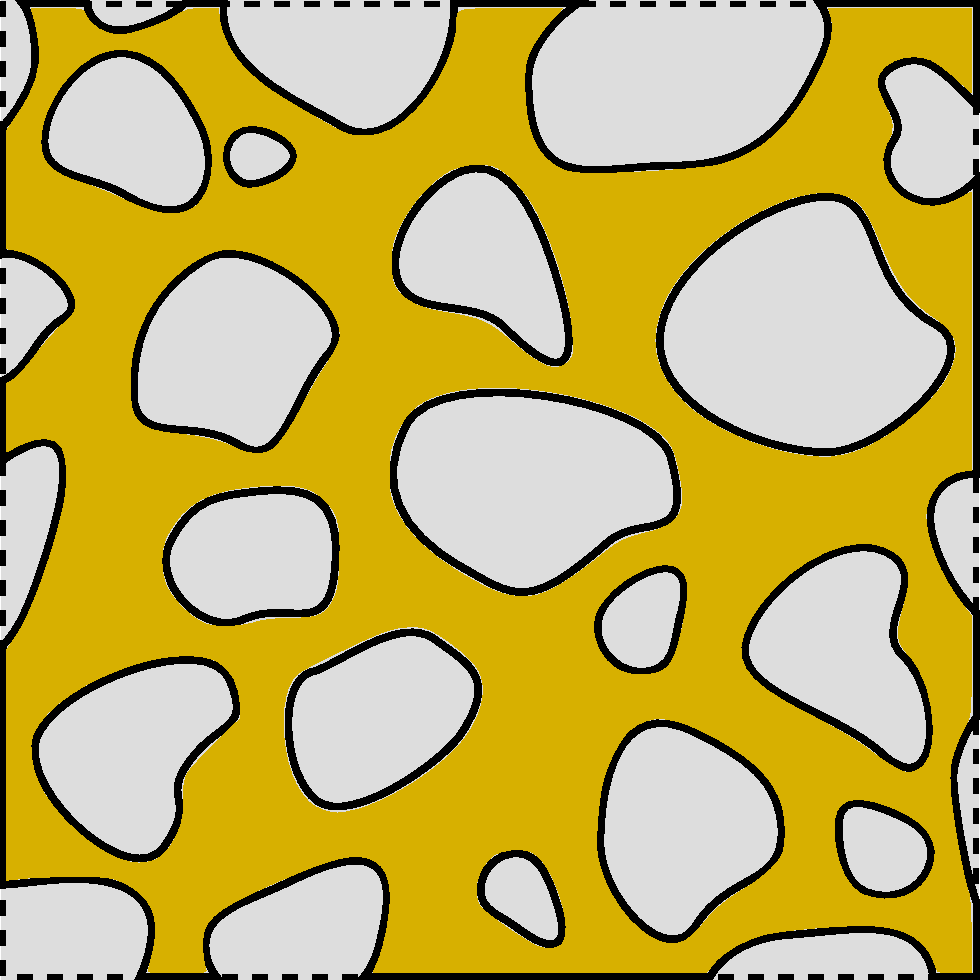
\includegraphics[scale=.3]{SwissCheeseFig}
%    };
% %\draw[<-, line width=.4mm] (1.6,5.0) .. controls +(up:0.5cm) and +(left:0.5cm) .. (2.5,5.7) node[right=1pt,black,text width=3cm,text badly ragged]{$\Gamma_\rve$};
% \draw[<-, line width=.4mm] (5.0,3.5) .. controls +(right:0.5cm) and +(left:0.5cm) .. (6.0,3.5) node[right,black]{$\Gamma_\rve$};
% \draw[<-, line width=.4mm] (4.6,2.) .. controls +(right:0.5cm) and +(left:0.5cm) .. (6.0,2.0) node[right,black]{$\Gamma_\rve^\pore$};
% %\draw[-*, line width=.4mm] (-1.0,1.5) node[left=-2.0cm,black,text width=3cm,text badly ragged]{$\Omega_{\rve,i}^\mathrm{p}$} .. controls +(right:0.5cm) and +(left:1.cm) .. (0.6,1.1);
% \draw[-*, line width=.4mm] (-1.0,2.1) node[left,black]{$\Omega_\rve^\particle$} .. controls +(right:0.5cm) and +(left:1.cm) .. (0.6,2.1);
% \draw[-*, line width=.4mm] (-1.0,3.1) node[left,black]{$\Omega_\rve^\pore$} .. controls +(right:0.5cm) and +(left:1.cm) .. (1.2,3.1);
% %\draw[<-, line width=.4mm] (4.6,1.7) .. controls +(right:0.5cm) and +(left:0.5cm) .. (6.0,1.0) node[right=1pt,black,text width=3cm,text badly ragged]{$\partial\Omega_{\rve,i}^\text{p}$};
% \end{tikzpicture}
% %}
% \caption{Generic micro-heterogeneous material consisting of inclusions in matrix (example)}
% \label{Figure1}
% \end{figure}

We consider a model material as follows: The stress is decomposed in terms of deviator and pressure as $\ts{\sigma} = \ts{\sigma}_\dev - p\ts{I}$.
With the kinematic definition $\devop[\ta v]\defeq[\ta v\outerp\diff]^\sym-\frac{1}{3}[\ta v\cdot\diff]\ts{I}$, we introduce the constitutive relations
%------------------------------------------------------------------------------------------------------------
\begin{equation}
    \ts{\sigma}_\dev = \hat{\ts{\sigma}}_\dev(\devop[\ta v]), \quad
    \ta v\cdot\diff = \hat{e}(p)
\label{eq201}
\end{equation}
%------------------------------------------------------------------------------------------------------
Hence, $\hat{\ts{\sigma}}_\dev(\bullet)$ and $\hat{e}(\bullet)$ denote suitable constitutive functions.
In the simplest case of viscous fluid, we have $\hat{\ts{\sigma}}_\dev(\ts{d}_\dev)=2\mu\ts{d}_\dev$ and $\hat{e}(p)=- C p$, where $\mu(\ta{x}), C(\ta{x})$ for $\ta{x}\in\Omega$ may fluctuate strongly.
Moreover, intrinsic incompressibility is defined as $\hat{e}(p)=0$ for any value of $p$.
In the case of flow problems, $C = 0$ is the only reasonable choice, however, the more general form is kept to illustrate the similarity between the fine-scale and macro-scale problem.

In this setting, the instantaneous velocity is solved for at any given time, and explicit time-integration is used to drive the deformations.


%%%%%%%%%%%%%%%%%%%%%%%%%%%%%%%%%%%%%%%%%%%%%%%%%%%%%%%%%%%%%%%%%%%%%%%%%%%%%%%%%%%%%%%%%%%%%%%5
\section{Surface tension}

\begin{figure}[th!]
    \centering
    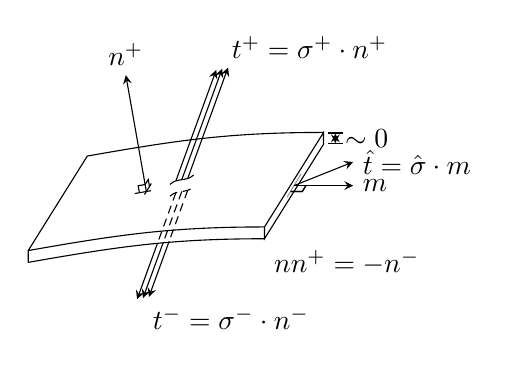
\begin{tikzpicture}[>=stealth,scale=1.5]
 \coordinate (A) at (0,0);
 \coordinate (B) at (2,0.2);
 \coordinate (C) at (2.5,1);
 \coordinate (D) at (0.5,0.8);
 \coordinate (At) at (0,-0.1);
 \coordinate (Bt) at (2,0.1);
 \coordinate (Ct) at (2.5,0.9);

 \draw (A) to[out=10,in=180] (B)
      (At) to[out=10,in=180] (Bt)
      (Bt) -- (B) -- (C) coordinate[midway] (E) -- (Ct) -- cycle
      (At) -- (A) -- (D) to[out=10,in=180] (C);

 % Binormal m
 \draw[draw=black!40] (E)++(0,-0.05)++(-0.06,-0.1) -- +(0.12,0.2);
 \draw[->] (E)++(0,-0.05) -- +(0.5,0) node[right]{$\ta{m}$};
 \draw[->] (E)++(0,-0.05) -- +(0.5,0.2) node[right]{$\hat{\ta{t}}=\hat{\ts{\sigma}}\cdot\ta{m}$};
 \draw (E)++(-0.03,-0.1) -- ++(0.1,0) -- +(0.03,0.05);
 \draw (E)++(0,-0.05)++(-0.03,-0.05) -- ++(0.1,0) -- +(0.03,0.05);

 
 % Normal
 \coordinate (n) at (1,0.5);
 \draw[->] (n) -- +(100:1) node[above]{$\ta{n}^+$};
 \draw (n)++(190:0.06) -- ++(100:0.06) -- +(190:-0.06);
 \draw (n)++(190:0.1) -- +(190:-0.14);
 \draw (n)++(58:0.05) -- ++(100:0.06) -- +(58:-0.05);
 \draw (n)++(58:0.08) -- +(58:-0.11);
 %\draw (n)++(190:0.06) -- ++(58:0.05) -- ++(190:-0.06);
 
 % Traction +
 \draw[->] (1.3,0.6) -- +(70:1) node[above right]{$\ta{t}^+ = \ts{\sigma}^+\cdot\ta{n}^+$};
 \draw[->] (1.35,0.61) -- +(70:1);
 \draw[->] (1.25,0.59) -- +(70:1);
 \draw (1.2,0.56) to[out=45,in=-135] (1.4,0.64);

 % Traction -
 \draw[densely dashed] (1.3,0.5) -- +(-110:0.46) coordinate (tmin); \draw[->] (tmin) -- +(-110:0.5) node[below right]{$\ta{t}^- =  \ts{\sigma}^-\cdot\ta{n}^-$};
 \draw[densely dashed] (1.35,0.51) -- +(-110:0.46) coordinate (tmin); \draw[->] (tmin) -- +(-110:0.5);
 \draw[densely dashed] (1.25,0.49) -- +(-110:0.46) coordinate (tmin); \draw[->] (tmin) -- +(-110:0.5);
 \draw[densely dashed] (1.2,0.46) to[out=45,in=-135] (1.4,0.54);

 % Thickness
 \draw[|<->|] ([xshift=0.1cm]C) -- ([xshift=0.1cm]Ct) node[midway,right] {$\sim 0$};

 % Definition
 \node[right] at (2,-0.1) {$\ta{n} \defeq \ta n^+ = -\ta n^-$};
\end{tikzpicture}
    \caption{Thin shell representing a surface with in-plane forces due to ``surface tension''.}
    \label{fig:surfacestress}
\end{figure}
A vital part of the simulation is the modeling of surface tension which acts as the ``driving force'' for liquid-phase sintering.
An extensive theory on boundary energy potentials has been developed by Steinmann \cite{steinmann_boundary_2008}, which has served as the basis for the surface tension modeling in this work.
In short; equilibrium across a surface $\mathcal{S}$ represented by a thin shell bounded by the curve $\mathcal{C}$, as in Figure~\ref{fig:surfacestress} can be stated as:
\begin{align}
    \ta{t}^+ + \ta{t}^- + \ta{t}_\surf &= \ta{0} \quad \text{on} \,\, \mathcal{S} \quad \text{with } \ta{t}_\surf \defeq \hat{\ts\sigma}\cdot\hat{\diff}
\label{eq103KR}\\
    \sum_i \hat{\ta t}_i &= \ta{0} \quad \text{on} \,\, \mathcal{C}
\label{eq104KR}
\end{align}
where $\hat\diff \defeq \diff - [\diff\cdot\ta n]\ta n$.
For an isotropic surface potential one obtains $\hat{\ts\sigma} = \gamma_\surf[\ts I-\ta n\outerp\ts n]$ and the common expression for the surface traction representing surface tension is obtained:
\begin{align}
 \ta t_\surf = -\kappa \gamma_\surf \ta n,\quad \text{where}\quad \kappa \defeq \ts n\cdot\hat\diff
\end{align}
where $\kappa$ is the Gaussian curvature.


%%%%%%%%%%%%%%%%%%%%%%%%%%%%%%%%%%%%%%%%%%%%%%%%%%%%%%%%%%%%%%%%%%%%%%%%%%%%%%%%%%%%%%%%%%%%%%%5
\section{Weak format of fine scale problem}
We are now in the position to formulate the strong format of the fine-scale problem under standard quasistatic conditions:
%------------------------------------------------------------------------------------------------------------
\begin{subequations}\label{eq1}
\begin{alignat}{2}
    -\left[\hat{\ts{\sigma}}_\dev(\devop[\ta v])-p\ts{I}\right]\cdot\diff & = \ta{f} &&\,\,\text{in}\,\, \Omega^\particle
 \label{eq1a} \\
    -\ta v\cdot\diff +  \hat{e}(p) & = 0 &&\,\,\text{in}\,\, \Omega^\particle
\label{eq1b} \\
    \ta v & = \ta v_\prescribed &&\,\,\text{on}\,\, \Gamma^\Dirichlet
\label{eq1c} \\
    \ta{t}\defeq\left[\hat{\ts{\sigma}}_\dev(\devop[\ta v])-p\ts{I}\right]\cdot\ta{n} & = \ta t_\prescribed &&\,\,\text{on}\,\, \Gamma^\Neumann
\label{eq1d} \\
    \ta{t}\defeq\left[\hat{\ts{\sigma}}_\dev(\devop[\ta v])-p\ts{I}\right]\cdot\ta{n} & =\ta{t}_\surf &&\,\,\text{on}\,\, \Gamma^\pore
\label{eq1surf}
\end{alignat}
\end{subequations}
%-----------------------------------------------------------------------------------------------------
The corresponding weak format is: Find $\ta v\in\set{V}, p\in\set{P}$ s.t.
%----------------------------------------------------------------------------------------------------------------
\begin{subequations}\label{eq2}
\begin{alignat}{3}
    a(\ta v;\delta\ta v) + b(p,\delta\ta v) &= l^\pore(\delta\ta v) + l(\delta\ta v) &\quad& \forall \delta\ta v &&\in \set{V}^{0}
\label{eq2a} \\
    b(\delta p,\ta v) + c^*(p;\delta p) &= 0 &\quad& \forall \delta p &&\in \set{P}
\label{eq2b}
\end{alignat}
\end{subequations}
%----------------------------------------------------------------------------------------------------------------------
where
%----------------------------------------------------------------------------------------------------------------
\begin{align}
    a(\ta{v};\ta{w}) &\defeq
    \int_{\Omega^\particle}  \devop[\ta{w}]\dprod \hat{\ts{\sigma}}_\dev(\devop[\ta{v}]) \dif V
\label{eq3a} \\
    b(q,\ta{v}) &\defeq
    - \int_{\Omega^\particle}  q\,\ta{v}\cdot\diff \dif V
\label{eq3b} \\
    c^*(q;r) &\defeq
    \int_{\Omega^\particle}  r\,\hat{e}(q) \dif V
\label{eq3c} \\
    l^\pore(\ta{v}) &\defeq -\int_{\Gamma^\pore} \gamma_\surf \hat{\ta I} \dprod [\ta{v}\outerp\diff] \dif S 
\label{eq3d} \\
    l(\ta{v}) &\defeq \int_{\Omega^\particle} \ta{v}\cdot\ta{f} \dif V + \int_{\Gamma^\Neumann} \ta{v}\cdot \ta t_\prescribed \dif S
\label{eq3e}
\end{align}

%%%%%%%%%%%%%%%%%%%%%%%%%%%%%%%%%%%%%%%%%%%%%%%%%%%%%%%%%%%%%%%%%%%%%%%%%%%%%%%%%%%%%%%%%%%%%%%%%%%%%%%%%%%
%%%%%%%%%%%%%%%%%%%%%%%%%%%%%%%%%%%%%%%%%%%%%%%%%%%%%%%%%%%%%%%%%%%%%%%%%%%%%%%%%%%%%%%%%%%%%%%%%%%%%%%%%%%
%%%%%%%%%%%%%%%%%%%%%%%%%%%%%%%%%%%%%%%%%%%%%%%%%%%%%%%%%%%%%%%%%%%%%%%%%%%%%%%%%%%%%%%%%%%%%%%%%%%%%%%%%%%
\section{Numerical aspects}
The mixed $(\ta v,p)$-formulation requires some form of stabilized elements for use with FEM. In this thesis, Taylor-Hood elements (quadratic velocity, linear velocity) and Mini-elements (linear pressure, linear velocity plus a bubble function) have been implemented.
Surface tension has been implemented according to \cref{eq3d}.

During the FE-simulation, the mesh eventually becomes very distorted, in particular at sharp corners subjected to surface tension.
In order to approach full density, pores need to shrink to the point of vanishing. 
A remeshing strategy was developed in \refpaper{A} to deal with this issue.
The assumption of viscous flow alleviates part of the problem, as there are no state variables to map to the new mesh.
Only the updated surfaces needs to be tracked, but that alone is a considerable effort as there are multiple phases and boundary conditions and the remeshing strategy needs to be fully automated.

% \subsection{RVE-problem}
% \begin{figure}[th!]
%   \centering
%   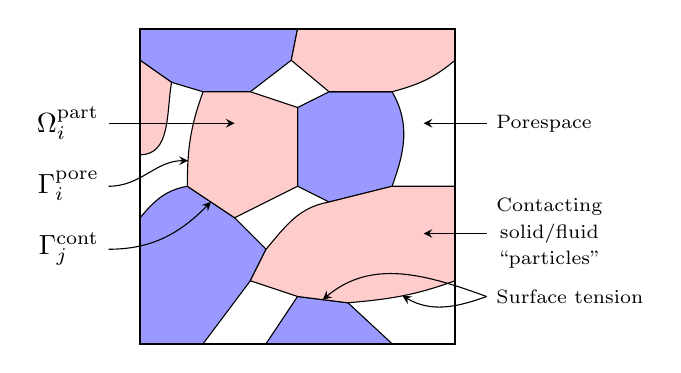
\begin{tikzpicture}[>=stealth,scale=4]
  \coordinate (A) at (0.35,0.2);
  \coordinate (B) at (0.4,0.3);
  \coordinate (C) at (0.3,0.4);
  \coordinate (D) at (0.15,0.5);
  \coordinate (E) at (0.66,0.13);
  \coordinate (F) at (0.6,0.45);
  \coordinate (G) at (0.8,0.5);
  \coordinate (H) at (0.5,0.5);
  \coordinate (I) at (0.5,0.75);
  \coordinate (J) at (0.6,0.8);
  \coordinate (K) at (0.8,0.8);
  \coordinate (L) at (0.35,0.8);
  \coordinate (M) at (0.5,1);
  \coordinate (N) at (0,0.9);
  \coordinate (O) at (0.1,0.83);
  \coordinate (P) at (0.5,0.15);
  \coordinate (Q) at (0.48,0.9);
  \coordinate (R) at (0.2,0.8);
  
  % Region 1 particles 
  \draw[fill=blue!40] 
  (0,0) -- (0.2,0) -- (A) -- (B) -- (C) -- (D) to[out=190,in=50] (0,0.4) -- cycle %A
  (0.4,0) -- (P) -- (E) -- (0.8,0) -- cycle %B
  (F) -- (G) to[out=70,in=-60] (K) -- (J) -- (I) -- (H) -- cycle %C
  (M) -- (Q) -- (L) -- (R) -- (O) -- (N) -- (0,1) -- cycle %D
  ;

  % Region 2 particles
  \draw[fill=red!20]
  (0,0.6) to[out=0,in=-100] (O) -- (N) -- cycle %E
  (D) to[out=90,in=-110] coordinate[near start] (surf3) (R) -- (L) -- (I) -- (H) -- (C) -- (D) coordinate[midway] (surf4) %F
  (M) -- (Q) -- (J) -- (K) to[out=15,in=-140] (1,0.9) -- (1,1) -- cycle %G
  (1,0.2) to[out=-160,in=5] coordinate[midway] (surf1) (E) -- (P) coordinate[midway] (surf2) -- (A) -- (B) to[out=50,in=-170] (F) -- (G) -- (1,0.5) -- cycle %H
  ;

  \draw[thick] (0,0) rectangle (1,1);

  % Annotations
  \draw[<-] (0.9,0.7) -- (1.1,0.7) node[right,font=\scriptsize] {Porespace};
  \draw[<-] (0.9,0.35) -- (1.1,0.35) node[right,font=\scriptsize] {\shortstack{Contacting\\solid/fluid\\``particles''}};
  \draw[<-] (surf1) to[out=-30,in=-160] (1.1,0.15) node[right,font=\scriptsize] {Surface tension};
  \draw[<-] (surf2) to[out=40,in=160] (1.1,0.15); % extra arrow
  \draw[<-] (surf3) to[out=180,in=0] (-0.1,0.5) node[left] {$\Gamma_i^{\mathrm{pore}}$};
  \draw[<-] (surf4) to[out=-135,in=0] (-0.1,0.3) node[left] {$\Gamma_j^{\mathrm{cont}}$};
  \draw[<-] (0.3,0.7) to[out=180,in=0] (-0.1,0.7) node[left] {$\Omega_i^{\mathrm{part}}$};
\end{tikzpicture}
%   \caption{Microstructure of porous particulate material with sintering particles in contact.}
%   \label{fig:micro}
% \end{figure}
% The fundamental microconstituents of the subscale are defined in Figure~\ref{fig:micro}.
% Surface tension could be considered on all boundaries; $\Gamma_i^{\mathrm{pore}}$ and $\Gamma_j^{\mathrm{cont}}$; however, it is assumed to be zero on $\Gamma_j^{\mathrm{cont}}$ in all the numerical examples in the appended papers.
% %
% \begin{figure}[H]
%     \centering
%     \begin{tikzpicture}[>=latex,scale=2] % Use this to scale the image. Text is always normal-size
  \def\particleradius{1.05} % Adjust this to change the contact size.
  \pgfmathsetmacro{\contactsize}{sqrt(\particleradius^2-1)} % Automatically calculated.
  \begin{scope}[very thick]
  	\draw[clip] (-1,-1) rectangle (1,1);
  	\draw[clip]
  		(-1,-1) circle (\particleradius)
 		( 1,-1) circle (\particleradius)
 		(-1, 1) circle (\particleradius)
   		( 1, 1) circle (\particleradius);
  	\fill[fill=black!10] (-1,-1) rectangle (1,1);
  \end{scope}
  % Markers
  \foreach \q in {0,90,180,270} { \draw[rotate=\q] (1-\contactsize,-0.05) -- +(0,0.1); }
  \draw[dashed,gray] (-1.1,0) -- (1.1,0) (0,-1.1) -- (0,1.1);
  % Annotations
  %\node[below] at (0,0) {$\Omega_\Box^p(0)$};
  \draw[|<->|] (-1,-1.4) -- (1,-1.4) node[midway,above] {$L_\Box(0)$};
  \draw[<->|] (-1,-0.05) -- +(\contactsize,0) node[midway,below] {$a_0$};
  \node at (0.6,-0.6) {$\Omega_\Box^{\mathrm{part}}(0)$};
  \draw[<-] (1,-0.5) -- +(0.2,0) node[right] {$\Gamma_\Box(0)$};
  \draw[<-] (1,1) ++(-135:\particleradius) -- +(0.00,0.15) node[above right] {$\Gamma_\Box^{\mathrm{pore}}(0)$};
  
  %\draw[use as bounding box] (-1.7,-1.5) rectangle (1.7,1.1);
  %\useasboundingbox (-1.7,-1.5) (1.7,1.1);
  % Transformation arrow (makes the picture very unaligned)
  %\draw[->] (1.5,0) to[out=45,in=-150] (2,0);% +(135:0.1) -- (2,0) -- +(-135:0.1);
\end{tikzpicture}

%     %\subfloat[$t = 0$]{\begin{tikzpicture}[>=latex,scale=2] % Use this to scale the image. Text is always normal-size
  \def\particleradius{1.05} % Adjust this to change the contact size.
  \pgfmathsetmacro{\contactsize}{sqrt(\particleradius^2-1)} % Automatically calculated.
  \begin{scope}[very thick]
  	\draw[clip] (-1,-1) rectangle (1,1);
  	\draw[clip]
  		(-1,-1) circle (\particleradius)
 		( 1,-1) circle (\particleradius)
 		(-1, 1) circle (\particleradius)
   		( 1, 1) circle (\particleradius);
  	\fill[fill=black!10] (-1,-1) rectangle (1,1);
  \end{scope}
  % Markers
  \foreach \q in {0,90,180,270} { \draw[rotate=\q] (1-\contactsize,-0.05) -- +(0,0.1); }
  \draw[dashed,gray] (-1.1,0) -- (1.1,0) (0,-1.1) -- (0,1.1);
  % Annotations
  %\node[below] at (0,0) {$\Omega_\Box^p(0)$};
  \draw[|<->|] (-1,-1.4) -- (1,-1.4) node[midway,above] {$L_\Box(0)$};
  \draw[<->|] (-1,-0.05) -- +(\contactsize,0) node[midway,below] {$a_0$};
  \node at (0.6,-0.6) {$\Omega_\Box^{\mathrm{part}}(0)$};
  \draw[<-] (1,-0.5) -- +(0.2,0) node[right] {$\Gamma_\Box(0)$};
  \draw[<-] (1,1) ++(-135:\particleradius) -- +(0.00,0.15) node[above right] {$\Gamma_\Box^{\mathrm{pore}}(0)$};
  
  %\draw[use as bounding box] (-1.7,-1.5) rectangle (1.7,1.1);
  %\useasboundingbox (-1.7,-1.5) (1.7,1.1);
  % Transformation arrow (makes the picture very unaligned)
  %\draw[->] (1.5,0) to[out=45,in=-150] (2,0);% +(135:0.1) -- (2,0) -- +(-135:0.1);
\end{tikzpicture}
\label{fig:4particle_rve_a}}
%     %\subfloat[$t > 0$]{\begin{tikzpicture}[>=latex,scale=1.6] % Use this to scale the image. Text is always normal-size
  \def\particleradius{1.05} % Adjust this to change the contact size.
  \draw[thick,fill=black!10,even odd rule] (0.9,-1.1) 
  	to[out=190,in=10] (-1.1,-0.9)
  	to[out=80,in=-110] (-0.9,1.1)
  	to[out=10,in=-160] (1.1,1.1)
  	to[out=-100,in=60] (0.9,-1.1) -- cycle
  	(-0.1,-0.5) to[out=180,in=-45] (-0.2,-0.15) to[out=135,in=-90]
  	(-0.5,0)    to[out=90,in=-135] (-0.15,0.15)  to[out=45,in=-180]  
  	(0.1,0.5)   to[out=0,in=135]   (0.2,0.15)   to[out=-45,in=90] coordinate[near start] (GammaF)
  	(0.5,0)     to[out=-90,in=45]  (0.15,-0.15)  to[out=-135,in=0] (-0.1,-0.5) -- cycle;
  % Markers
  \draw[dashed,gray] (-1.1,0) to[out=5,in=-175] (1.1,0) (-0.2,-1.1) -- (0.2,1.1);
  % Annotations
  \node at (0.5,-0.6) {$\Omega_\Box(t)$};
  \draw[<-] (GammaF) -- +(0.00,0.15) node[above right] {$\Gamma_\Box^{\mathrm{pore}}(t)$};
\end{tikzpicture}\label{fig:4particle_rve_b}}
%     \caption{Idealized initial configuration of the RVE in 2D consisting of circular particles in a square lattice.}
%     \label{fig:4particleRVE}
% \end{figure}
% %
% In the simplest form, the RVE is idealized to a unit cell with four contacting circular particles.
% The size of the initial contact surface after compaction is represented by the length $a_0$.
% 
% During the FE-simulation of the RVE, the mesh becomes very distorted, in particular when the sharp contact is rapidly rounded off and when the pores vanish.
% A remeshing strategy was developed in \refpaper{A} to deal with this issue.

%For the homogenization of the RVE, Dirichlet boundary condition was chosen due to its simplicity. Periodic boundary conditions were not considered to to its difficulty in relation to remeshing and Neumann boundary condition remain as a future work.


%%%%%%%%%%%%%%%%%%%%%%%%%%%%%%%%%%%%%%%%%%%%%%%%%%%%%%%%%%%%%%%%%%%%%%%%%%%%%%%%%%%%%%%%%%%%%%%%%%%%%%%%%%%
%%%%%%%%%%%%%%%%%%%%%%%%%%%%%%%%%%%%%%%%%%%%%%%%%%%%%%%%%%%%%%%%%%%%%%%%%%%%%%%%%%%%%%%%%%%%%%%%%%%%%%%%%%%
%%%%%%%%%%%%%%%%%%%%%%%%%%%%%%%%%%%%%%%%%%%%%%%%%%%%%%%%%%%%%%%%%%%%%%%%%%%%%%%%%%%%%%%%%%%%%%%%%%%%%%%%%%%
%%%%%%%%%%%%%%%%%%%%%%%%%%%%%%%%%%%%%%%%%%%%%%%%%%%%%%%%%%%%%%%%%%%%%%%%%%%%%%%%%%%%%%%%%%%%%%%%%%%%%%%%%%%
\chapter{Formulation of the two-scale problem}

\begin{figure}[htpb!]
\centering
\begin{tikzpicture}
 \node at (0,0) {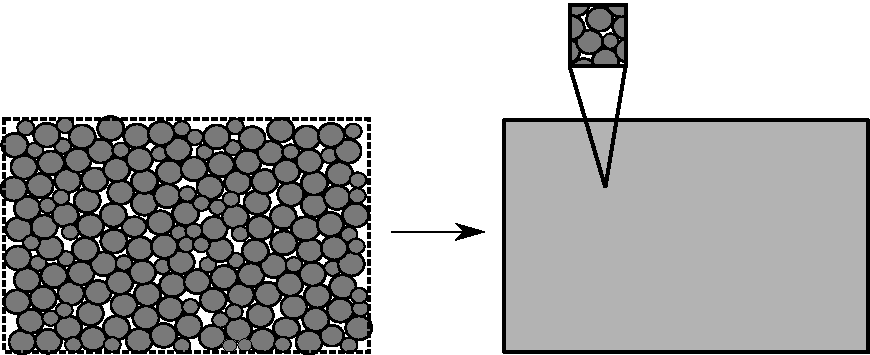
\includegraphics[scale=0.6]{figures/Homogenization.pdf}};
 \node at (2.5,1.5) {RVE};
 \node at (-2.5,-2.2) {Fine-scale};
 \node at (2.5,-2.2) {Macroscale};
 \node at (0,0) {VCH};
 \draw[latex-] (-4.1,0.1) -- ++(-1,0) node[left] {$\Omega^\particle$};
 \draw[latex-] (-4.2,-0.15) to (-5.1,0.1);
 \draw[latex-] (4.4,0) -- ++(1,0) node[right] {$\Gamma^\Neumann$, $\Gamma^\Dirichlet$};
 \node at (2.5,0) {$\Omega$};
\end{tikzpicture}
\caption{Homogenization of a ``green body''. Particles are not to scale.}
\label{fig:homogenization}
\end{figure}


As the amount of detail in the in the fine scale problem exceeds the computational, we must use homogenization. 
Variationally Consistent Homogenization (VCH) will be used to obtain the two-scale problem, as illustrated in \cref{fig:homogenization}.
By applying a split of both $\ta v$ and $p$ (not the only possible choice, as can be seen in \refpaper{A}) we then choose suitable definitions of the macroscopic response variables $\bar{\ts\sigma}_\dev$ and $\bar{e}$ in order to obtain a macroscopic problem as follows
\begin{subequations}\label{eq:prototype_macro}
\begin{alignat}{2}
 -[\bar{\ts\sigma}_\dev\{\devop[\bar{\ta v}], \bar{p}\} -\bar{p}\ts I]\cdot\diff &= \bar{\ta f} &&\text{ in } \Omega
\\
 -\bar{\ta v}\cdot\diff + \bar{e}\{\devop[\bar{\ta v}], \bar{p}\} &= 0 &&\text{ in } \Omega
\\
 \bar{\ta v} &= \bar{\ta v}_\prescribed &&\text{ on } \Gamma_\Dirichlet
\\
 \bar{\ta t} &= \bar{\ta t}_\prescribed &&\text{ on } \Gamma_\Neumann
\end{alignat}
\end{subequations}


%%%%%%%%%%%%%%%%%%%%%%%%%%%%%%%%%%%%%%%%%%%%%%%%%%%%%%%%%%%%%%%%%%%%%%%%%%%%%%%%%%%%%%%%%%%%%%%%%%%%%%%%%%%
%%%%%%%%%%%%%%%%%%%%%%%%%%%%%%%%%%%%%%%%%%%%%%%%%%%%%%%%%%%%%%%%%%%%%%%%%%%%%%%%%%%%%%%%%%%%%%%%%%%%%%%%%%%
%%%%%%%%%%%%%%%%%%%%%%%%%%%%%%%%%%%%%%%%%%%%%%%%%%%%%%%%%%%%%%%%%%%%%%%%%%%%%%%%%%%%%%%%%%%%%%%%%%%%%%%%%%%
%%%%%%%%%%%%%%%%%%%%%%%%%%%%%%%%%%%%%%%%%%%%%%%%%%%%%%%%%%%%%%%%%%%%%%%%%%%%%%%%%%%%%%%%%%%%%%%%%%%%%%%%%%%
\section{Variationally Consistent Homogenization (VCH)}

Throughout all included papers, the VCH method has been applied.
We introduce the abbreviated notation $z = (\ta v, p) \in \set{Z} = \set V \times \set P$, where $\set Z$ represents the space of fine-scale (non-homogenized) solutions.
Similarly, $\set Z^0 = \set V^0 \times \set P$ is the test space and where each $\ta v\in \set V^0$ vanishes on the Dirichlet part of the boundary.

The abstract formulation of a multifield problem based on a given set of balance (or constraint) equations may conveniently be abbreviated in abstract form as the residual equation
%-------------------------------------------------------------------------------------------------------------------------------
\begin{align}
 R(z; \delta z) \defeq R_\Omega(z; \delta z) + R_\Gamma(z;\delta z) = 0\quad \forall\;\delta z\in \set Z^0
\label{eq:A1}
\end{align}
VCH is applied in all appended papers.
No explicit reference to the specific character of the underlying problem is made in this section.

%%%%%%%%%%%%%%%%%%%%%%%%%%%%%%%%%%%%%%%%%%%%%%%%%%%%%%%%%%%%%%%%%%%%%%%%%%%%%%%%%%%%%%%%%%%%%%%%%%%%%%%%%%%
%%%%%%%%%%%%%%%%%%%%%%%%%%%%%%%%%%%%%%%%%%%%%%%%%%%%%%%%%%%%%%%%%%%%%%%%%%%%%%%%%%%%%%%%%%%%%%%%%%%%%%%%%%%
%%%%%%%%%%%%%%%%%%%%%%%%%%%%%%%%%%%%%%%%%%%%%%%%%%%%%%%%%%%%%%%%%%%%%%%%%%%%%%%%%%%%%%%%%%%%%%%%%%%%%%%%%%%
%%%%%%%%%%%%%%%%%%%%%%%%%%%%%%%%%%%%%%%%%%%%%%%%%%%%%%%%%%%%%%%%%%%%%%%%%%%%%%%%%%%%%%%%%%%%%%%%%%%%%%%%%%%
\subsection{VMS-approach -- Scale separation and homogenization}

Classical model-based homogenization can be formulated in the spirit of the Variational MultiScale method (VMS), cf.\ \cite{hughes_variational_1998}, \cite{larson_adaptive_2007}.

%-------------------------------------------------------------------------------------------------------------------------------

A multiscale formulation of \cref{eq:A1} is defined by the hierarchical split $\set Z = \set Z^\macro \oplus \set Z^\fluct$, where $\set Z^\macro$ contains smooth macroscale functions and $\set Z^\fluct$ is the hierarchical complement of $\set Z^\macro$ that, typically, represents the fine-scale features.
It is assumed that each $z\in \set Z$ can be split uniquely as $z = z^\macro + z^\fluct$ such that $z^\macro \in \set Z^\macro$ and $z^\fluct \in \set Z^\fluct$.
Therefore, solve $z^\macro \in \set Z^\macro$, $z^\fluct \in \set Z^\fluct$ such that \cref{eq:A1} can be represented by the set of equations
%------------------------------------------------------------------------------------------------------------------------------------------------
\begin{subequations}\label{eq:A2}
\begin{alignat}{3}
\label{eq:A2a} & R(z^\macro + z^\fluct; \delta z^\macro) &&= 0 \quad &&\forall\;\delta z^\macro \in \set Z^{\macro,0}\\
\label{eq:A2b} & R(z^\macro + z^\fluct; \delta z^\fluct) &&= 0       &&\forall\;\delta z^\fluct \in \set Z^{\fluct}
\end{alignat}
\end{subequations}
%-----------------------------------------------------------------------------------------------------------------------------
Without introducing further assumptions (approximations), the dimension of the original problem has not changed, i.e.\ \cref{eq:A2} represent two global problems whose solution requires the same computational effort as does \cref{eq:A1}.
In order to reduce the problem dimension based on homogenization (via the assumption of scale separation), we introduce the following key assumptions:

\begin{itemize}
\item The integrands in the pertinent volume integrals are replaced by a running volume average on RVE's
such that, typically, the residual in \cref{eq:A2a} can be rewritten in terms of the contributions defined on each RVE as
%--------------------------------------------------------------------------------------------------------------------------
\begin{align}
\label{eq:A106} R_\Omega(z;\delta z) = \int_\Omega R_\rve(z;\delta z)(\bar{\ta x})\dif\Omega
\end{align}
%--------------------------------------------------------------------------------------------------------------------------
where $R_\rve$ is the RVE-residual that is localized to the Representative Volume Element (RVE).
In practice (in FE-analysis), quadrature is used such that the evaluation of $R_\rve$ is carried out only in the Gauss points.

Furthermore, for the sake of simplicity we assume smoothness of boundary terms, such that $R_\Gamma(z; \delta z^\macro) \approx R_\Gamma(z^\macro;\delta z^\macro)$, i.e.\ no boundary homogenization is necessary.

\item Local approximations for the fluctuation field $z^\fluct$ are introduced in the spirit of VMS.
This means that $z^\fluct \approx \tilde{z}^\fluct\{z^\macro\}\in\set{Z}_\rve^{\fluct}$ is the \emph{approximate} solution of the fine-scale 
equation \cref{eq:A2b} for given $z^\macro$, i.e.\ \cref{eq:A2b} is replaced by ``closed'' RVE-problems (in the macroscale quadrature points) associated with a particular choice of boundary conditions on $\Omega_\rve$.
%In this paper we obtain such ``closed'' RVE-problems by choosing  weakly periodic boundary conditions.
\end{itemize}
Returning to \cref{eq:A2a}, we now replace this problem by the approximate, homogenized, problem
%---------------------------------------------------------------------------------------------------------------------------------------------
\begin{multline}
\label{eq:A3} R(z^\macro+\tilde{z}^\fluct\{z^\macro\};\delta z^\macro) = \int_\Omega R_\rve(z^\macro+\tilde{z}^\fluct\{z^\macro\};\delta z^\macro)(\bar{\ta x})\dif\Omega
 \\
 + R_\Gamma(z^\macro, \delta z^\macro) = 0 \quad \forall\;\delta z^\macro \in \set Z^{\macro,0}
\end{multline}
%--------------------------------------------------------------------------------------------------------------------------------
which has the same dimension as \cref{eq:A2a}.
We note that \cref{eq:A3} represents a valid homogenization problem for any given choice of $\set{Z}_\rve^{\fluct}$; however, to preserve typical Galerkin properties, such as symmetry of the macroscale tangent operator when such symmetry is inherent in the underlying fine-scale problem, it is crucial to satisfy the VCMC.


%%%%%%%%%%%%%%%%%%%%%%%%%%%%%%%%%%%%%%%%%%%%%%%%%%%%%%%%%%%%%%%%%%%%%%%%%%%%%%%%%%%%%%%%%%%%%%%%%%%%%%%%%%%
%%%%%%%%%%%%%%%%%%%%%%%%%%%%%%%%%%%%%%%%%%%%%%%%%%%%%%%%%%%%%%%%%%%%%%%%%%%%%%%%%%%%%%%%%%%%%%%%%%%%%%%%%%%
%%%%%%%%%%%%%%%%%%%%%%%%%%%%%%%%%%%%%%%%%%%%%%%%%%%%%%%%%%%%%%%%%%%%%%%%%%%%%%%%%%%%%%%%%%%%%%%%%%%%%%%%%%%
%%%%%%%%%%%%%%%%%%%%%%%%%%%%%%%%%%%%%%%%%%%%%%%%%%%%%%%%%%%%%%%%%%%%%%%%%%%%%%%%%%%%%%%%%%%%%%%%%%%%%%%%%%%
\subsection{Variationally Consistent Macrohomogeneity Condition (VCMC)}

We shall assume that there exists a potential $\Pi(z)$ such that \cref{eq:A3} represents the stationary point of $\Pi(z)$, i.e.\ it is assumed that
%---------------------------------------------------------------------------------------------------------------------------------------
\begin{align}
\label{eq:A4} R(z;\delta z) = \Pi'(z;\delta z) \defeq \frac{\dif}{\dif\epsilon}\Pi(z+\epsilon\delta z)|_{\epsilon = 0} = 0\quad \forall\;\delta z \in \set Z^0
\end{align}
%------------------------------------------------------------------------------------------------------
Next, we introduce the crucial \emph{approximation} (restriction) $z \approx z^\macro + \tilde{z}^\fluct\{z^\macro\}$ before evaluation of the stationarity conditions, whereby we obtain
%---------------------------------------------------------------------------------------------------------------------------------------
\begin{align}
\label{eq:A5} \Pi_{z^\macro}'\{z^\macro;\delta z^\macro\} & \defeq
\frac{\dif}{\dif\epsilon}\Pi(z^\macro+\epsilon \delta z^\macro+\tilde{z}^\fluct\{z^\macro+\epsilon \delta z^\macro\})|_{\epsilon = 0} \nonumber \\
& =
R(z^\macro + \tilde{z}^\fluct\{z^\macro\}; \delta z^\macro + (\tilde{z}^\fluct)'\{z^\macro;\delta z^\macro\}) = 0\quad \forall\;\delta z^\macro\in\set Z^{\macro,0}
\end{align}
%------------------------------------------------------------------------------------------------------------------------------------------
where $(\tilde{z}^\fluct)'\{z^\macro;\delta z^\macro\}$ denotes the sensitivity (or directional derivative) of $\tilde z^\fluct$ for a variation $\delta z^\macro$ of the macroscale solution $z^\macro$.
Hence, the choice of test function in \cref{eq:A5} is restricted as compared to \cref{eq:A4}, and this restriction represents a ``generalized Galerkin property'' in terms of the underlying macroscale functions in $\set Z^\macro$.
Moreover, and most importantly, \cref{eq:A5} is completely equivalent to the homogenized problem \cref{eq:A3} if it is possible, for any given $z^\macro\in\set Z^{\macro}$, to satisfy the constraint
%---------------------------------------------------------------------------------------------------------------------------------------------
\begin{align}
\label{eq:A6a} R(z^\macro + \tilde z^\fluct\{z^\macro\}; (\tilde{z}^\fluct)'\{z^\macro;\dif z^\macro\}) = 0\quad \forall\;\dif z^\macro\in\set Z^{\macro,0}(z^\macro)
\end{align}
%-------------------------------------------------------------------------------------------------------------------------------------------------
or, equivalently,
%---------------------------------------------------------------------------------------------------------------------------------------------
\begin{align}
\label{eq:A6b} R(z^\macro + \tilde z^\fluct\{z^\macro\}; \dif\tilde{z}^\fluct) = 0\quad \forall\;\dif\tilde{z}^\fluct\in\tilde{\set Z}'^{\fluct}(z^\macro)
\end{align}
%-------------------------------------------------------------------------------------------------------------------------------------------------
where the test space $\tilde{\set Z}'^{\fluct}(z^\macro)$, which is the tangent space to the approximation space, is defined as
%----------------------------------------------------------------------------------------------------------------
\begin{align}
    \tilde{\set{Z}}'^{\fluct}(z^\macro)\defeq\{\set{Z}^\fluct\ni \dif z^\fluct = (\tilde{z}^\fluct)'\{z^\macro;\dif z^\macro\},\,
    \dif z^\macro\in \set{Z}^{\macro,0}\}
\label{eq:A6c}
\end{align}
%----------------------------------------------------------------------------------------------------------------------
Hence, any $\dif \tilde{z}^\fluct\in\tilde{\set{Z}}'^{\fluct}(z^\macro)$ is a sensitivity of the fluctuation field $\tilde{z}^\fluct$ for a differential change of the macroscale field $z^\macro$ within the considered RVE.
It is computed from the tangent problem that is associated with the RVE-problem.
We refer to \cref{eq:A6a} or \cref{eq:A6b} as a ``Variationally Consistent (generalized) Macrohomogeneity Condition'' (VCMC).
Obviously, a sufficient condition for these identities to hold true is to require the RVE-residual to vanish on each RVE (in each quadrature point), i.e.\ to ensure that
%--------------------------------------------------------------------------------------------------------------------------------------
\begin{align}
\label{eq:A8} R_\rve(z^\macro + \tilde z^\fluct\{z^\macro\};(\tilde{z}^\fluct)'\{z^\macro;\delta z^\macro\}) = 0\quad \forall\;z^\macro,\delta z^\macro\in\set Z^{\macro}|_{\Omega_\rve}\times\set Z^{\macro,0}|_{\Omega_\rve}
\end{align}
%----------------------------------------------------------------------------------------------------------------------------------------------
An even stronger condition is to require that $R_\rve(z;\delta z^\fluct) = 0$ for \emph{any} $\delta z^\fluct$ in a given set of functions that is defined locally for the considered RVE without requiring any implicit (or explicit) 
coupling to the sensitivity field $(\tilde{z}^\fluct)'\{z^\macro;\delta z^\macro\}$, which obviously defines a restricted choice of test functions.
In such a case, the VCMC can be identified as precisely the classical Hill-Mandel macrohomogeneity condition.

Finally, we remark that the VCMC ensures that the macroscale tangent operator becomes symmetrical, since it holds that
%---------------------------------------------------------------------------------------------------------------------------------------
\begin{align}
\label{eq:A9} R'(z;\delta z_1,\delta z_2) = \Pi''(z;\delta z_1,\delta z_2) \defeq \frac{\dif}{\dif\epsilon}\Pi'(z+\epsilon\delta z_2;\delta z_1)|_{\epsilon=0}\quad \forall\;\delta z_1,\delta z_2 \in \set Z^0
\end{align}
%------------------------------------------------------------------------------------------------------
With the introduced approximation $z^\fluct \approx \tilde{z}^\fluct\{z^\macro\}$, the test functions in \cref{eq:A9} are chosen as
%---------------------------------------------------------------------------------------------------------------------------------------
\begin{align}
\label{eq:A10} \delta z_i \approx \delta z_i^\macro + (\tilde{z}^\fluct)'\{z^\macro;\delta z_i^\macro\} \quad \forall\;\delta z_i^\macro\in\set Z^{\macro,0}, \,\, i=1,2
\end{align}
%------------------------------------------------------------------------------------------------------------------------------------------

\section{Choice of the hierarchical split}
The common theme throughout the series articles is the treatment of macroscopic incompressibility.
In \refpaper{A}, the split ($\ta v = \ta v^\macro + \ta v^\fluct$) was only introduced to the velocity field, while the for the incompressibility condition was solved in each RVE independently (i.e.\ $p^\macro = 0$, $p = p^\fluct$).
By choosing to do so, only the momentum balance equation is obtained at the macroscopic level.
In the RVE problem the constraints are placed for a unique decomposition, e.g.\ $\homgen{\ta v \outerp\diff} = \bar{\ta v}\outerp\diff$ (or equivalently $\homgen{\ta v^\fluct\outerp\diff} = \ts 0$) for a first order expansion of the velocity field.
However, at the incompressible limit, when all microconstituents are intrinsically incompressible and no pore space exist, it is necessary to satisfy part of this constraint weakly.
In \refpaper{B} this is done by algebraic manipulation of the FE\textsuperscript{2} procedure derived in \refpaper{A}, while in \refpaper{C} and \refpaper{D} this is obtained directly as part of the homogenization procedure.


For an RVE with no pores or surface tension, as in \refpaper{C}, the prolongation of the macroscopic fields $\bar{\ta v}$ (or equivalently $\bar{\ta u}$) and $\bar{p}$ are as expected;
First order Taylor expansion of the velocity field, and zeroth order expansion for the pressure field
\begin{align}
 \ta v^\macro &= \bar{\ta v} + [\bar{\ta v}\outerp\diff]\cdot[\ta x - \bar{\ta x}]
\\
 p^\macro &= \bar{p}
\end{align}
where we require that in each RVE
\begin{align}
 \homgen{\ta v\outerp\diff} &= \bar{\ta v}\outerp\diff
\\
 \homgen{p} &= \bar{p}
\end{align}

However, in the case when pores and surface tension are present, as in \refpaper{D}, it is necessary to carefully choose the prolongation in such a way that we obtain the desired (simple) macroscale formulation:
\begin{align}
 \ta v^\macro = \bar{\ta v} + [\bar{\ta v}\outerp\diff]\cdot[\ta x - \bar{\ta x}]
\\
 p^\macro = \frac{\volume}{|\Omega_\rve^\particle|}[\bar{p} + \frac23\shomgen{\gamma_\surf}]
\end{align}
where we now require that in each RVE
\begin{align}
 \int_{\Gamma_\rve}\ta v\outerp\ta n\dif S = \bar{\ta v}\outerp\diff
\\
 \homgen{p} - \frac23\homgen{\gamma_\surf} = \bar{p}
\end{align}
However, by rewriting the problem and always connect the scales through the RVE-boundary, we obtain a simple relation that holds true both \refpaper{C} and \refpaper{D};
\begin{align}
 \frac{1}{\volume}\int_{\Gamma_\rve}\ta v\outerp\ta n\dif S &= \bar{\ta v}\outerp\diff
\\
 \frac{1}{\volume}\int_{\Gamma_\rve}\ta t\outerp[\ta x-\bar{\ta x}]\dif S &= \bar{\ts\sigma} \implies \int_{\Gamma_\rve}\ta t\cdot[\ta x-\bar{\ta x}]\dif S = \bar{p}
\end{align}


%%%%%%%%%%%%%%%%%%%%%%%%%%%%%%%%%%%%%%%%%%%%%%%%%%%%%%%%%%%%%%%%%%%%%%%%%%%%%%%%%%%%%%%%%%%%%%%%%%%%%%%%%%%
\section{Numerical aspects}

In \refpaper{B--C} the macroscale problems, as shown in \cref{eq:prototype_macro}, will also require stabilization and the Taylor-Hood elements are is the obvious choice.
While computationally much more expensive than traditional macroscopic material models, the FE\textsuperscript{2} procedure allows for trivial parallelization w.r.t.\ macroscale integration points.




%%%%%%%%%%%%%%%%%%%%%%%%%%%%%%%%%%%%%%%%%%%%%%%%%%%%%%%%%%%%%%%%%%%%%%%%%%%%%%%%%%%%%%%%%%%%%%%%%%%%%%%%%%%
%%%%%%%%%%%%%%%%%%%%%%%%%%%%%%%%%%%%%%%%%%%%%%%%%%%%%%%%%%%%%%%%%%%%%%%%%%%%%%%%%%%%%%%%%%%%%%%%%%%%%%%%%%%
%%%%%%%%%%%%%%%%%%%%%%%%%%%%%%%%%%%%%%%%%%%%%%%%%%%%%%%%%%%%%%%%%%%%%%%%%%%%%%%%%%%%%%%%%%%%%%%%%%%%%%%%%%%
%%%%%%%%%%%%%%%%%%%%%%%%%%%%%%%%%%%%%%%%%%%%%%%%%%%%%%%%%%%%%%%%%%%%%%%%%%%%%%%%%%%%%%%%%%%%%%%%%%%%%%%%%%%
\chapter{Summary of Appended Papers}

\begin{itemize}
 \item \textbf{\refpaper{A}: \citefield{ohman_computational_2012}{title}}.
Liquid phase sintering of particle agglomerates is simulated as the viscous deformation of particle-particle contact, whereby the single driving force is the surface tension on the particle/pore interface.
Particles are modeled as purely viscous fluids (with no elasticity). 
Computational homogenization is adopted for the RVE with Dirichlet boundary conditions.
A surface motion algorithm was developed that requires complete remeshing of the FE-mesh based on a ``maximum deformation'' criterion. 
Since the particles are intrinsically incompressible, the macroscopic compressibility is determined from shrinking porosity in the substructure.

The numerical examples include free sintering of an RVE and a fully coupled FE\textsuperscript{2}-simulation of a specimen with inhomogeneous initial distribution of porosity.

The FE\textsuperscript{2}-format (only valid for macroscopic compressibility) for the Dirichlet boundary condition is summarized in the following flowchart
\begin{center}
%  \tikzsetnextfilename{box1}
  \begin{tikzpicture}[node distance = 2cm, auto,scale=0.8, transform shape, >=latex']
    %\small
    %\tikzstyle{every node}=[font=\footnotesize]
    \tikzstyle{group}    = [rectangle, draw, thick, dashed, text width=6em, text centered, rounded corners]
    \tikzstyle{decision} = [diamond,   draw, fill=white, aspect=2, node distance=2.5cm, inner sep=2pt]
    \tikzstyle{block}    = [rectangle, draw, fill=white, text width=6em, text centered, rounded corners]
    \tikzstyle{line}     = [draw, ->]

    \draw [thick, dashed, fill=blue!10, rounded corners] (-4.5,0.5) rectangle ( 1.9,-7.8);
    \draw [thick, dashed, fill=red!10,  rounded corners] ( 3.8,0.5) rectangle (10.1,-7.8);
    \node [below right, inner sep=10pt] at (-4.5,0.5) { \textbf{\large Macro} };
    \node [below left,  inner sep=10pt] at (10.1,0.5) { \textbf{\large RVE} };

    % Place nodes
    \node [block] (init) {Initial guess};
    \node [block, below of=init, text width=8em, node distance=1.5cm] (residual) {Compute residual from (12)};
    \node [decision, below of=residual,node distance=2cm] (convergence) {Converged?};
    \node [block, below of=convergence, node distance=2.3cm] (stop) {Finish step};
    \node [block, left of=stop, node distance=3cm] (update) {Newton iteration: Compute tangent};
    % Draw edges
    \path [line] (init) -- (residual) node[midway] {$\bar{\ta{v}}$};
    \path [line] (residual) -- (convergence);
    \path [line] (convergence) -- node {False} (update);
    \path [line] (convergence) -- node {True} (stop);
    \path [line] (update) |- node[near start,right] {$\bar{\ta{v}}$} (residual);

    % Place nodes
    \node [block, right of=init, node distance=5.6cm] (rve_init) {Initial guess};
    \node [block, below of=rve_init, text width=8em, node distance=1.5cm] (rve_residual) {Compute residual from (16)};
    \node [decision, below of=rve_residual, node distance=2cm] (rve_convergence) {Converged?};
    \node [block, below of=rve_convergence, node distance=2.3cm] (rve_stop) {Post-process $\bar{\ts\sigma}$};
    \node [block, right of=rve_stop, node distance=3cm] (rve_update) {Newton iteration: Compute tangent};
    % Sensitivity problem
    \node [block, below of=rve_stop, node distance=1.3cm] (rve_sensitivity) {Sensitivity problem};
    
    % Draw edges
    \path [line] (rve_init) -- (rve_residual) node[midway] {$\ta{v}^\fluct,p$};
    \path [line] (rve_residual) -- (rve_convergence);
    \path [line] (rve_convergence) -- node {False} (rve_update);
    \path [line] (rve_convergence) -- node {True} (rve_stop);
    \path [line] (rve_update) |- node[right, near start] {$\ta{v}^\fluct,p$} (rve_residual);

    \path [line] (residual.east) ++(0, 0.2cm) -- ++(0.7cm,0) |- node [below,pos=0.65] {$\bar{\ts d}_\dev, \bar{e}$} (rve_init);
    % Draw this backwards in order to get exact alignments
    \path [line, <-] (residual.east) ++(0,-0.2cm) -- ++(0.7cm,0) |- node [below,pos=0.65] {$\bar{\ts\sigma}_\dev, \bar{p}$} (rve_stop);

    \path [line] (rve_sensitivity) -| node[below, pos=0.10] {$\bar{\tf E}$} (update);
\end{tikzpicture}

% \includegraphics{box1.pdf}
% \caption{Flow-chart of FE\textsuperscript{2}-format valid only for macroscopic compressibility}
% \label{fig:box1}
\end{center}

 \item \textbf{\refpaper{B}: \citefield{ohman_computational_2013}{title}}.
Liquid phase sintering of particle agglomerates is modeled on the mesoscale as the viscous deformation of particle-particle contact, whereby the single driving force is the surface tension on the particle/pore interface.
On the macroscale, a quasistatic equilibrium problem allows for the prediction of the shrinkage of the sintering body. 
The present paper presents a novel FE\textsuperscript{2} formulation of the two-scale sintering problem allowing for the transition to zero porosity, implying macroscale incompressibility.
The seamless transition from compressibility to incompressibility on the macroscale is accomplished by introducing a mixed variational format.
This has consequences also for the formulation of the mesoscale problem, that is complemented with an extra constraint equation regarding the prolongation of the volumetric part of the macroscopic rate-of-deformation.

The numerical example shows the sintering of a single representative volume element (RVE), which is sheared beyond the point where the porosity vanishes while subjected to zero macroscopic pressure.

The FE\textsuperscript{2}-format (modified to handle seamless transition from macroscopic compressibility to incompressibility) for the Dirichlet boundary condition is summarized in the following flowchart
\begin{center}
%  \tikzsetnextfilename{box2}
  \begin{tikzpicture}[node distance = 2cm, auto,scale=0.8, transform shape, >=latex']
    %\small
    %\tikzstyle{every node}=[font=\footnotesize]
    \tikzstyle{group}    = [rectangle, draw, thick, dashed, text width=6em, text centered, rounded corners]
    \tikzstyle{decision} = [diamond,   draw, fill=white, text width=6em, text centered, aspect=2, node distance=2.5cm, inner sep=2pt]
    \tikzstyle{block}    = [rectangle, draw, fill=white, text width=6em, text centered, rounded corners]
    \tikzstyle{line}     = [draw, ->]

    \draw [thick, dashed, fill=blue!10, rounded corners] (-4.5,0.5) rectangle ( 1.9,-7.8);
    \draw [thick, dashed, fill=red!10,  rounded corners] ( 3.8,0.5) rectangle (10.1,-7.8);
    \node [below right, inner sep=10pt] at (-4.5,0.5) { \textbf{\large Macro} };
    \node [below left,  inner sep=10pt] at (10.1,0.5) { \textbf{\large RVE} };

    % Place nodes
    \node [block] (init) {Initial guess};
    \node [block, below of=init, text width=8em, node distance=1.5cm] (residual) {Compute residual from (20)};
    \node [decision, below of=residual,node distance=2cm] (convergence) {Converged?};
    \node [block, below of=convergence, node distance=2.3cm] (stop) {Finish step};
    \node [block, left of=stop, node distance=3cm] (update) {Newton iteration: Compute tangent};
    % Draw edges
    \path [line] (init) -- (residual) node[midway] {$\bar{\ta{v}},\bar{p}$};
    \path [line] (residual) -- (convergence);
    \path [line] (convergence) -- node {False} (update);
    \path [line] (convergence) -- node {True} (stop);
    \path [line] (update) |- node[near start,right] {$\bar{\ta{v}},\bar{p}$} (residual);

    % Place nodes
    \node [block, right of=init, node distance=5.6cm] (rve_init) {Initial guess};
    \node [block, below of=rve_init, text width=8em, node distance=1.5cm] (rve_residual) {Compute residual from (22)};
    \node [decision, below of=rve_residual, node distance=2cm] (rve_convergence) {Converged?};
    \node [block, below of=rve_convergence, node distance=2.3cm] (rve_stop) {Post-process $\bar{\ts\sigma}_\dev$};
    \node [block, right of=rve_stop, node distance=3cm] (rve_update) {Newton iteration: Compute tangent};
    % Sensitivity problem
    \node [block, below of=rve_stop, node distance=1.3cm] (rve_sensitivity) {Sensitivity problem (36)};
    
    % Draw edges
    \path [line] (rve_init) -- (rve_residual) node[midway] {$\ta{v}^\fluct,p, \bar{e}, \ta t, \bar{\ts\sigma}_\dev$};
    \path [line] (rve_residual) -- (rve_convergence);
    \path [line] (rve_convergence) -- node {False} (rve_update);
    \path [line] (rve_convergence) -- node {True} (rve_stop);
    \path [line] (rve_update) |- node[right, near start, text width=1.5em] {$\ta{v}^\fluct,p$, $\bar{e}, \ta t, \bar{\ts\sigma}_\dev$} (rve_residual);

    \path [line] (residual.east) ++(0, 0.2cm) -- ++(0.7cm,0) |- node [below,pos=0.65] {$\bar{\ts d}_\dev, \bar{p}$} (rve_init);
    % Draw this backwards in order to get exact alignments
    \path [line, <-] (residual.east) ++(0,-0.2cm) -- ++(0.7cm,0) |- node [below,pos=0.65] {$\bar{\ts\sigma}_\dev, \bar{e}$} (rve_stop);

    \path [line] (rve_sensitivity) -| node[below, pos=0.10] {$\substack{\displaystyle\bar{\tf E}_\ded,\bar{\ts C}_\ded \\ \displaystyle\bar{\ts E}_\dep,\bar{C}_\dep}$} (update);
\end{tikzpicture}

% \includegraphics{box2.pdf}
% \caption{Flow-chart of FE\textsuperscript{2}-format for seamless transition from macroscopic compressibility to incompressibility}
% \label{fig:box1}
\end{center}


 \item \textbf{\refpaper{C}: \citefield{ohman_variationally_2014}{title}}.
In this work, a mixed displacement-pressure formulation for elasticity is considered as the prototype problem.
Variationally Consistent Homogenization is directly used to derive the macroscale problem, and the Variationally Consistent Macrohomogeneity condition is used to determine the RVE problem.
Dirichlet, Neumann, and (weakly) periodic boundary conditions for the RVE's are derived, and the Dirichlet and Neumann boundary conditions are shown to be bounds for the periodic boundary condition.

The numerical examples show the convergence rate of the Neumann and Dirichlet boundary conditions for a series of 3D Statistical Volume Elements (SVE's).
A final example shows the influence of the compressibility of the microconstituents on the homogenized macroscopic shear modulus.


The FE\textsuperscript{2}-format for the weakly periodic boundary condition is summarized in the following flowchart
\begin{center}
%  \tikzsetnextfilename{box3}
  \begin{tikzpicture}[node distance = 2cm, auto,scale=0.8, transform shape]
    %\small
    %\tikzstyle{every node}=[font=\footnotesize]
    \tikzstyle{group}    = [rectangle, draw, thick, dashed, text width=6em, text centered, rounded corners]
    \tikzstyle{decision} = [diamond,   draw, fill=white, text width=4em, text centered, node distance=2.5cm, inner sep=0pt]
    \tikzstyle{block}    = [rectangle, draw, fill=white, text width=6em, text centered, rounded corners]
    \tikzstyle{line}     = [draw, -latex']

    \draw [thick, dashed, fill=blue!10, rounded corners] (-4.5,0.5) rectangle ( 1.9,-7.8);
    \draw [thick, dashed, fill=red!10,  rounded corners] ( 3.8,0.5) rectangle (10.4,-7.8);
    \node [below right, inner sep=10pt] at (-4.5,0.5) { \textbf{\large Macro} };
    \node [below left,  inner sep=10pt] at (10.1,0.5) { \textbf{\large RVE} };

    % Place nodes
    \node [block] (init) {Initial guess};
    \node [block, below of=init, text width=8em, node distance=1.5cm] (residual) {Compute residual};
    \node [decision, below of=residual,node distance=2cm] (convergence) {Check conv.};
    \node [block, below of=convergence, node distance=2.3cm] (stop) {Finish step};
    \node [block, left of=stop, node distance=3cm] (update) {Newton iteration: Compute tangent};
    % Draw edges
    \path [line] (init) -- (residual) node[midway] {$\bar{\ta{u}},\bar{p}$};
    \path [line] (residual) -- (convergence);
    \path [line] (convergence) -- node {\footnotesize False} (update);
    \path [line] (convergence) -- node {\footnotesize True} (stop);
    \path [line] (update) |- node[near start,right] {$\bar{\ta{u}},\bar{p}$} (residual);

    % Place nodes
    \node [block, right of=init, node distance=5.6cm] (rve_init) {Initial guess};
    \node [block, below of=rve_init, text width=8em, node distance=1.5cm] (rve_residual) {Compute residual};
    \node [decision, below of=rve_residual, node distance=2cm] (rve_convergence) {Check conv.};
    \node [block, below of=rve_convergence, node distance=2.3cm] (rve_stop) {Post-process $\bar{\ts\sigma}_\dev$};
    \node [block, right of=rve_stop, node distance=3cm] (rve_update) {Newton iteration: Compute tangent};
    % Sensitivity problem
    \node [block, below of=rve_stop, node distance=1.3cm] (rve_sensitivity) {Sensitivity problem};
    
    % Draw edges
    \path [line] (rve_init) -- (rve_residual) node[midway] {$\ta{u},p,\bar{e},\ta{t}$};
    \path [line] (rve_residual) -- (rve_convergence);
    \path [line] (rve_convergence) -- node {\footnotesize False} (rve_update);
    \path [line] (rve_convergence) -- node {\footnotesize True} (rve_stop);
    \path [line] (rve_update) |- node[right, near start] {$\ta{u},p,\bar{e},\ta{t}$} (rve_residual);

    \path [line] (residual.east) ++(0, 0.2cm) -- ++(0.7cm,0) |- node [below,pos=0.65] {$\bar{\ts \epsilon}_\dev, \bar{p}$} (rve_init);
    % Draw this backwards in order to get exact alignments
    \path [line, latex'-] (residual.east) ++(0,-0.2cm) -- ++(0.7cm,0) |- node [below,pos=0.65] {$\bar{\ts\sigma}_\dev, \bar{e}$} (rve_stop);

    \path [line] (rve_sensitivity) -| node[below, pos=0.10] {$\substack{\displaystyle\bar{\tf E}_\ded,\bar{\ts C}_\ded \\ \displaystyle\bar{\ts E}_\dep,\bar{C}_\dep}$} (update);
\end{tikzpicture}

% \includegraphics{box3.pdf}
% \caption{Flow-chart of FE\textsuperscript{2}-format ...}
% \label{fig:box3}
\end{center}


 \item \textbf{\refpaper{D}: \citefield{ohman_new_2014}{title}}.
The final work in this thesis extends the Variationally Consistent Homogenization of the mixed formulation presented in \refpaper{C} with the mesoscale modeling found in \refpaper{A} and \refpaper{B}.
In particular, it is shown that the Dirichlet boundary condition becomes equivalent to that in \refpaper{C}.
Also highlighted in this paper is that the surface tension may also have contribution to the deviatoric part of the macroscopic stress, whereas traditional models for sintering only accounts for volumetric macroscopic ``sintering stress''.
The deviatoric contribution to the macroscopic stress is naturally captured by the RVE-problems as part of the homogenization procedure.

The numerical examples show transient behavior of the Neumann and Dirichlet boundary conditions for a 2D RVE subject to free sintering.
A 3D microstructure with porespace and surface tension compares the effective macroscale properties between the Dirichlet, Neumann and weakly periodic boundary condition.

The FE\textsuperscript{2}-format for the weakly periodic boundary condition is summarized in the following flowchart
\begin{center}
%  \tikzsetnextfilename{box4}
  \begin{tikzpicture}[node distance = 2cm, auto,scale=0.8, transform shape]
    %\small
    %\tikzstyle{every node}=[font=\footnotesize]
    \tikzstyle{group}    = [rectangle, draw, thick, dashed, text width=6em, text centered, rounded corners]
    \tikzstyle{decision} = [diamond,   draw, fill=white, text width=4em, text centered, node distance=2.5cm, inner sep=0pt]
    \tikzstyle{block}    = [rectangle, draw, fill=white, text width=6em, text centered, rounded corners]
    \tikzstyle{line}     = [draw, -latex']

    \draw [thick, dashed, fill=blue!10, rounded corners] (-4.5,0.5) rectangle ( 1.9,-7.8);
    \draw [thick, dashed, fill=red!10,  rounded corners] ( 3.8,0.5) rectangle (10.4,-7.8);
    \node [below right, inner sep=10pt] at (-4.5,0.5) { \textbf{\large Macro} };
    \node [below left,  inner sep=10pt] at (10.1,0.5) { \textbf{\large RVE} };

    % Place nodes
    \node [block] (init) {Initial guess};
    \node [block, below of=init, text width=8em, node distance=1.5cm] (residual) {Compute residual};
    \node [decision, below of=residual,node distance=2cm] (convergence) {Check conv.};
    \node [block, below of=convergence, node distance=2.3cm] (stop) {Finish step};
    \node [block, left of=stop, node distance=3cm] (update) {Newton iteration: Compute tangent};
    % Draw edges
    \path [line] (init) -- (residual) node[midway] {$\bar{\ta{v}},\bar{p}$};
    \path [line] (residual) -- (convergence);
    \path [line] (convergence) -- node {\footnotesize False} (update);
    \path [line] (convergence) -- node {\footnotesize True} (stop);
    \path [line] (update) |- node[near start,right] {$\bar{\ta{v}},\bar{p}$} (residual);

    % Place nodes
    \node [block, right of=init, node distance=5.6cm] (rve_init) {Initial guess};
    \node [block, below of=rve_init, text width=8em, node distance=1.5cm] (rve_residual) {Compute residual};
    \node [decision, below of=rve_residual, node distance=2cm] (rve_convergence) {Check conv.};
    \node [block, below of=rve_convergence, node distance=2.3cm] (rve_stop) {Post-process $\bar{\ts\sigma}_\dev$};
    \node [block, right of=rve_stop, node distance=3cm] (rve_update) {Newton iteration: Compute tangent};
    % Sensitivity problem
    \node [block, below of=rve_stop, node distance=1.3cm] (rve_sensitivity) {Sensitivity problem};
    
    % Draw edges
    \path [line] (rve_init) -- (rve_residual) node[midway] {$\ta{v},p,\bar{e},\ta{t}$};
    \path [line] (rve_residual) -- (rve_convergence);
    \path [line] (rve_convergence) -- node {\footnotesize False} (rve_update);
    \path [line] (rve_convergence) -- node {\footnotesize True} (rve_stop);
    \path [line] (rve_update) |- node[right, near start] {$\ta{v},p,\bar{e},\ta{t}$} (rve_residual);

    \path [line] (residual.east) ++(0, 0.2cm) -- ++(0.7cm,0) |- node [below,pos=0.65] {$\bar{\ts d}_\dev, \bar{p}$} (rve_init);
    % Draw this backwards in order to get exact alignments
    \path [line, latex'-] (residual.east) ++(0,-0.2cm) -- ++(0.7cm,0) |- node [below,pos=0.65] {$\bar{\ts\sigma}_\dev, \bar{e}$} (rve_stop);

    \path [line] (rve_sensitivity) -| node[below, pos=0.10] {$\substack{\displaystyle\bar{\tf E}_\ded,\bar{\ts C}_\ded \\ \displaystyle\bar{\ts E}_\dep,\bar{C}_\dep}$} (update);
\end{tikzpicture}

% \includegraphics{box4.pdf}
% \caption{Flow-chart of FE\textsuperscript{2}-format ...}
% \label{fig:box4}
\end{center}

\end{itemize}


%%%%%%%%%%%%%%%%%%%%%%%%%%%%%%%%%%%%%%%%%%%%%%%%%%%%%%%%%%%%%%%%%%%%%%%%%%%%%%%%%%%%%%%%%%%%%%%
%%%%%%%%%%%%%%%%%%%%%%%%%%%%%%%%%%%%%%%%%%%%%%%%%%%%%%%%%%%%%%%%%%%%%%%%%%%%%%%%%%%%%%%%%%%%%%%
%%%%%%%%%%%%%%%%%%%%%%%%%%%%%%%%%%%%%%%%%%%%%%%%%%%%%%%%%%%%%%%%%%%%%%%%%%%%%%%%%%%%%%%%%%%%%%%
\chapter{Contributions of the thesis}
\begin{itemize}
 \item VCH homogenization of mixed v-p to v suitable for the sintering problem.
 \item Application of surface tracking algorithm and remeshing strategy suitable for free surface flows.
 \item Extending paper A to allow the particly incompressible FE\textsuperscript{2} simulation (paper B).
 \item VCH of (in)compressible elasticity in mixed u-p formulation.
  (investigating the influence of homogenized shear modulus w.r.t.\ bulk modulus) (paper C)
 \item VCH taking into account pores and surface tension. (paper A, B, D),
  (taking into account for the possibility of anisotropic sintering stress), ()
\end{itemize}


%%%%%%%%%%%%%%%%%%%%%%%%%%%%%%%%%%%%%%%%%%%%%%%%%%%%%%%%%%%%%%%%%%%%%%%%%%%%%%%%%%%%%%%%%%%%%%%
%%%%%%%%%%%%%%%%%%%%%%%%%%%%%%%%%%%%%%%%%%%%%%%%%%%%%%%%%%%%%%%%%%%%%%%%%%%%%%%%%%%%%%%%%%%%%%%
%%%%%%%%%%%%%%%%%%%%%%%%%%%%%%%%%%%%%%%%%%%%%%%%%%%%%%%%%%%%%%%%%%%%%%%%%%%%%%%%%%%%%%%%%%%%%%%
\chapter{Concluding remarks and Future work}

In this thesis a novel approach to simulate the sintering process as a problem of computational homogenization is presented, replacing the traditional macroscopic constitutive models.
With the new proposed homogenization procedure, we can ensure a seamless transition from the macroscopically compressible to the incompressible response, which is of vital importance when modeling sintering of particle composites.

Through rigorously applying VCH, we can ensure that the obtained multiscale problem is sound, and by further manipulation we can obtain a simpler and still consistent RVE-problem that retains the same strong form as the fine scale problem.
These manipulations allows for a straight forward FE-implementation.
The FE\textsuperscript{2} algorithm is freely available in the open source code OOFEM (cf.\ \cite{patzak_oofem_2000}) as free software.

For the homogenization procedure, pores on the RVE-boundaries remain complicated.
Weakly periodic and Neumann boundary conditions are not applicable, while Dirichlet boundary conditions constrains the closing of pores on the boundary.
A strongly periodic boundary condition could therefore be a necessity for these RVEs with pores, but makes it considerably harder to (re)generate a mesh.


There are also possible improvements of the subscale modeling, where the bulk- and surface-diffusion is still missing.
Due to limitations in the remeshing and post-processing software, the microstructural properties of the ``green body'', i.e.\ before the sintering process starts, have so far only been idealized to contacting spheres.
While these serve the need for demonstrating the homogenization procedure, they fail to capture a realistic microstructure, particularly that of WC-Co.

An attempt to address the large topological changes have been outlined in \refpaper{A}, but is lacking a robust 3D implementation.
Alternative methods such as level sets, volume fractions, or particle-FEM could offer a simpler numerical procedure for the fine-scale problem.

\end{document}
